\section{Inference}
\label{sec:inference}

Having completed the definition of the FFBM, we wish to leverage it 
to perform inference. Given a vertex-labelled graph $(A, X)$,
the goal is to sample from the posterior distribution
of $\theta$:
%
\begin{equation}
	\label{eqn:theta-target}
	\theta \sim p(\theta | A, X).
\end{equation}
%
We propose an iterative approach to obtain samples
$\theta^{(t)}$ from $p(\theta|A,X)$. We first draw samples $b^{(t)}$ 
from the block membership posterior distribution,
and then use each $b^{(t)}$ to obtain a corresponding
sample $\theta^{(t)}$:
%
\begin{align}
	b^{(t)} &\sim p ( b | A, X )  \label{eqn:b-samples},\\
	\theta^{(t)} &\sim p(\theta | X, b^{(t)} ). \label{eqn:theta-samples}
\end{align}
%
Both of these sampling steps can be implemented using
Markov chain Monte Carlo via a Metropolis-Hastings 
algorithm \cite{hastings-alg}, as a two-level Markov chain.

% We just need to define a proposal distribution $q(x, x')$ for proposing a move $x \rightarrow x'$ and be able to evaluate an un-normalised form of the target distribution, denoted $\pi(\cdot)$, point-wise. The proposed move is then accepted with probability $\alpha$ (equation \ref{eqn:mh-accept}) else it is rejected and we stay at $x$.
%
% \begin{equation}
	% \alpha(x, x') = \min \left( \frac{\pi(x') q(x', x)}{\pi(x) q(x, x')} , 1 \right)
	% \label{eqn:mh-accept}
% \end{equation}
%
% This accept-reject step ensures the resulting Markov Chain is in detailed balance with the target distribution $\pi(\cdot)$. 
% What we propose in equations \ref{eqn:b-samples} and \ref{eqn:theta-samples} is therefore implemented through a 2-level Markov chain. 
As we show in the following section, the resulting samples 
for $\theta^{(t)}$ are unbiased in the sense that the expectation of 
their distribution is the target posterior distribution:
%
\begin{equation}
\Expect_{b^{(t)}} \left[p \left( \theta | X, b^{(t)} \right) \right] = \sum_{b \in [B]^N} p(\theta | X, b) p(b | A, X) = \sum_{b \in [B]^N} p(\theta, b | A, X) = p(\theta | A, X).
\label{eqn:theta-unbiased}
\end{equation}
%
This is an example of a pseudo-marginal approach. Indeed, \citet{pseudo-marginal} show that~(\ref{eqn:theta-unbiased})
% the unbiased result in equation 
is sufficient to prove that, for large enough $t$, $\theta^{(t)} \sim \Expect_{b^{(i)}} \left[ p(\theta | X, b^{(t)})\right] = p(\theta 
| A, X)$, as required.
%  which is exactly the distribution we are targetting (equation \ref{eqn:theta-target}).

\begin{figure}[!h]
	\centering

	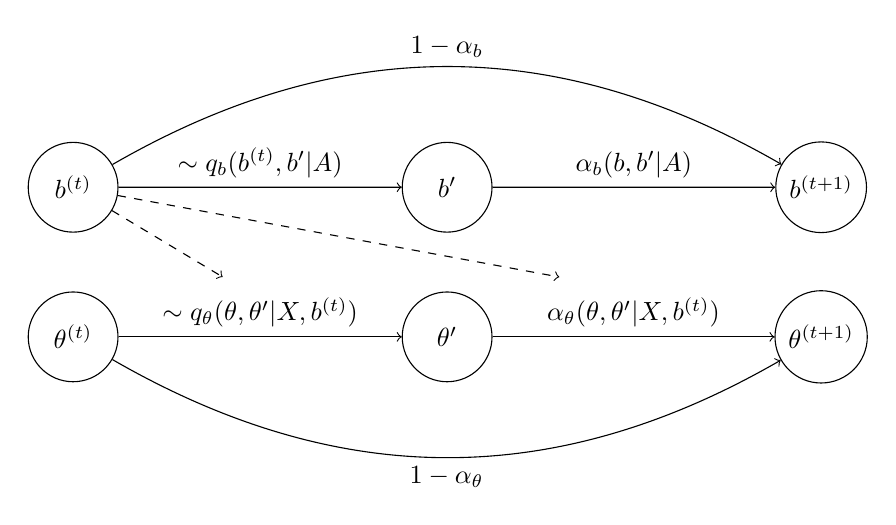
\begin{tikzpicture}[
		scale=0.95, every node/.style={transform shape},
		roundnode/.style={circle, draw=black, minimum size=12mm},
		squarednode/.style={rectangle, draw=black, minimum size=12mm}
		]
		% nodes
		\node[roundnode] (b0) at (0, 2) {$b^{(t)}$};
		\node[roundnode] (b1) at (5, 2) {$b'$};
		\node[roundnode] (b2) at (10, 2) {$b^{(t+1)}$};
		\node[roundnode] (t0) at (0, 0) {$\theta^{(t)}$};
		\node[roundnode] (t1) at (5, 0) {$\theta'$};
		\node[roundnode] (t2) at (10, 0) {$\theta^{(t+1)}$};
		
		% arrows
		\draw[->] (b0) to node[above] {$\sim q_b(b^{(t)}, b' | A)$} (b1);
		\draw[->] (b1) to node[above] {$\alpha_b (b, b' | A)$} (b2);
		\draw[->] (b0) [out=30, in=150] to node[above] {$1-\alpha_b$} (b2);
		
		\draw[->] (t0) to node[above] {$\sim q_\theta(\theta, \theta' | X, b^{(t)})$} (t1);
		\draw[->] (t1) to node[above] {$\alpha_\theta (\theta, \theta' | X, b^{(t)})$} (t2);
		\draw[->] (t0) [out=-30, in=-150] to node[below] {$1-\alpha_\theta$} (t2);
		
		\draw[dashed, ->] (b0) to (2, 0.8);
		\draw[dashed, ->] (b0) to (6.5, 0.8);
		
	\end{tikzpicture}
	\caption{Sampling sequence.}
	\label{fig:samp-sequence}
\end{figure}

The reason for splitting the Markov chain into two levels is that the summation over all latent states $b \in [B]^N$ required to directly compute the likelihood, $p(A| X, \theta) = \sum_{b \in [B]^N} p(A | b) P(b | X, \theta)$,
is intractable, as the sum involves $B^N$ terms. 
Figure \ref{fig:samp-sequence} shows an overview of the proposed method. 
The Metropolis-Hastings accept/reject probabilities 
for the proposed $b$ and $\theta$ samples are denoted $\alpha_b$ and
$\alpha_\theta$, respectively.
% We have introduced subscripts and conditionings to make explicit what variables each step utilises. 

Note the importance of the simplification in~(\ref{eqn:b-pseudo-prior}). 
As $p(b| X)$ in fact does not depend on $X$, 
knowing $X$ is not necessary in order to obtain samples
of the block membership vector $b$.
And on the other level, in order to obtain 
samples of the parameter vector $\theta$
we use only $b$ but not $A$, as $\theta$ and $A$ are
conditionally independent given $b$. 

\FloatBarrier
\clearpage
\subsection{Sampling block memberships}

We adopt the Markov chain Monte Carlo procedure of
\cite{Peixoto-MCMC},
which relies on writing the posterior in the following form:
%
\begin{equation}
	p(b | A, X) \propto p(A | b, X) \cdot p(b | X) = \pi_b(b).
\end{equation}
%
Now $\pi_b(\cdot)$ is the un-normalised target density,
which can be expressed as:
%  we wish to sample from for the $b$-chain. In other words, we 
% wish to construct a Markov chain that has $\pi_b(\cdot)$ 
% as its invariant distribution. We can break $\pi_b$ down as follows:
%
\begin{equation}
	\pi_b(b) = p(b|X) \sum_{\psi} \nolimits p(A , \psi | b, X) \\
	= p(b|X) p(A, \psi^* | b, X) \\
	= p(A | b, \psi^*) \cdot p(\psi^* | b) \cdot p(b | X).
\end{equation}
%
Since we are using the microcanonical SBM formulation, there is only one 
value of $\psi$ that is compatible with the given $(A, b)$ pair;
recall the constraints in~(\ref{eqn:sbm-constraints}). 
We denote this value $\psi^* = \{\psi_k^*, \psi_e^*\}$. Therefore, 
the summation over all $\psi$ reduces to just the single $\psi^*$ term.
% ; this is the power of the microcanonical formulation. 
We also define the microcanonical entropy of the configuration as,
%
\begin{equation}
	S(b) = - \log \pi_b(b) = - \Big( \log p(A | b, \psi^*) + \log p(\psi^*, b | X) \Big).
	\label{eqn:dl-form}
\end{equation}
%
This entropy can be thought of as the optimal
``description length'' of the graph. 
The exact form of the proposal $q_b$ is explored thoroughly in
\cite{Peixoto-MCMC} and not repeated here. There is a widely used 
library for Python made available under LGPL 
called \verb*|graph-tool| \cite{peixoto_graph-tool_2014}, 
which implements this algorithm. The only modification we make is in 
the block membership prior $p(b)$ that we replace with $p(b|X)=B^{-N}$, 
which cancels out in the MH accept-reject step as it is independent of $b$.

\subsection{Sampling feature-to-block generator parameters}
\label{s:sfb}

The invariant distribution we wish to target for the $\theta$ samples is the posterior of $\theta$ given the values of the pair $(X, b)$. 
We write this as,
%
\begin{equation}
	\pi_\theta(\theta) \propto p(\theta | X, b) \propto p(b | X, \theta) p(\theta) \propto  \exp \left( - U(\theta) \right),
	\label{eq:U}
\end{equation}
%
where we write $U(\theta)$ for the negative log-posterior. Let $y_{ij} \coloneqq \one \left\{ b_i = j \right\}$ and $a_{ij} \coloneqq \phi_j(x_i; \theta)$. 
Discarding constant terms, we can write $U(\theta)$ as,
%
\begin{equation}
	U(\theta) = \left( \sum_{i \in [N]} \sum_{j \in [B]} y_{ij} \log \frac{1}{a_{ij}} \right)
	+ \frac{1}{2\sigma_\theta^2} \|\theta\|^2 = N \cdot \Lcal(\theta) + \frac{1}{2\sigma_\theta^2} \|\theta\|^2;
	\label{eqn:U-form}
\end{equation}

See Appendix \ref{appdx:form-U} for the derivation. The function $U(\theta)$ is a typical objective function for neural network training. The first term is introduced by the likelihood. We collect it into $N \cdot \Lcal(\theta)$, which is the cross-entropy between the graph-predicted and feature-predicted block memberships summed over all vertices. 
The second, introduced by the prior, brings a form of regularisation, guarding against over-fitting. Unlike in many applications where the goal 
is to find the minimiser of $U(\theta)$, our goal is to draw samples from the posterior $\pi_\theta(\cdot) \propto \exp(-U(\cdot))$. We can use $\nabla U$ as a useful heuristic to bias our proposal towards regions of higher target density. We therefore adopt the Metropolis-adjusted Langevin algorithm (MALA) \cite{mala-tweedie}. Given the current sample $\theta$, we generate 
a new sample $\theta'$ as,
\begin{equation*}
	\theta' = \theta - h \nabla U(\theta) + \sqrt{2h} \cdot \xi,
\end{equation*}

where $\xi \sim \Gaussian(0, I)$ and $h$ is a step-size parameter 
which may vary with the sample index (see Appendix \ref{appdx:step-size}).
This leads to the proposal distribution,
\begin{equation*}
	q_\theta(\theta, \theta') \sim \Gaussian \left( \theta' ; \theta - h \nabla U(\theta), 2h I \right).
\end{equation*}

Without the injected noise term, MALA is equivalent to gradient descent. We require the noise term $\xi$ to fully explore the parameter space. 
The term $\nabla U$ has an easy to compute analytic form (derived in Appendix \ref{appdx:gradu}). By noting that $\theta = \{w_k\}_{k=1}^{B}$, we write the derivative with respect to each $w_k$ as,
%
\begin{equation}
	\frac{\partial U}{\partial w_k} = - \left( \sum_{i=1}^{N} \Big\{ \tilde{x}_i (y_{ik} - a_{ik}) \Big\} - \frac{w_k}{\sigma_\theta^2} \right).
	\label{eqn:U-derivative}
\end{equation}
%
After a proposed move is generated from $q_\theta$,
it is either accepted or rejected in the standard
Metropolis-Hastings accept/reject step.

\subsection{Sampling sequence}
\label{s:ss}

Up to this point, each $\theta^{(t)}$ update uses its corresponding $b^{(t)}$ sample. This means that the evaluation of $U(\theta)$ and $\nabla U(\theta)$ has high variance. This may lead to longer burn-in for the resulting Markov chain. The only link between $b^{(t)}$ and $\theta^{(t)}$ is in the evaluation of $U(\theta)$ and $\nabla U(\theta)$ which depends only on the matrix $y^{(t)}$ with entries $y_{ij}^{(t)} \coloneqq \one\{b_i^{(t)} = j\}$. We would rather deal with the expectation of each $y_{ij}^{(t)}$:
%
\begin{equation}
	\Expect \left[ y_{ij}^{(t)} \right] = \Expect_{b^{(t)}} \left[ \one(b_{i}^{(t)} = j) \right]
	= p(b_i = j | A, X).
\end{equation}
%
We can obtain an unbiased estimate for this quantity using 
the thinned $b$-samples after burn-in; the length of the
burn-in and the details of the thinning are described
in Appendix \ref{appdx:burn-in-thinning}.
Let $\Tcal_b$  denote the retained set of indices 
for the $b$-samples and $\Tcal_\theta$ similarly for the $\theta$-chain. 
The unbiased estimate for $y_{ij}^{(t)}$ using the 
restricted sample set $\Tcal_b$ is denoted $\hat{y}_{ij}$:
%
\begin{equation}
	\hat{y}_{ij} \coloneqq \frac{1}{|\Tcal_b|} \sum_{t \in \Tcal_b} y_{ij}^{(t)} = \frac{1}{|\Tcal_b|} \sum_{t \in \Tcal_b} \one\{b_i^{(t)} = j\}.
\end{equation}
%
The same matrix $\hat{y}$ is used in the update step
for each $\theta^{(t)}$.
This way, it is not necessary to run the $b$ and $\theta$ Markov chains 
concurrently. Instead, we run the $b$-chain to completion and use it 
to generate $\hat{y}$. This affords us the flexibility to vary the 
lengths of the $b$ and $\theta$-chains. Furthermore, the changeover 
from $y^{(t)}$ to $\hat{y}$ reduces the burn-in time for 
the $\theta$-chain by reducing the variance in the evaluation 
of $U$ and $\nabla U$. A detailed description of the overall 
algorithms is given in Appendix \ref{appdx:algorithms}.

\subsection{Dimensionality reduction}
\label{sec:dim-reduction}

Once the samples $\left\{ \theta^{(t)} \right\} \sim p(\theta | A, X)$
have been obtained, we can compute the empirical mean and standard deviation of each component of $\theta$. Switching back to matrix notation we define $\theta = W$, such that $W_{ij}$ is the weight component for block $i$ and feature $j$, we can define:
%
\begin{equation}
	\hat{\mu}_{ij} \coloneqq \frac{1}{|\Tcal_\theta|} \sum_{t \in \Tcal_\theta} W_{ij}^{(t)} \qquad \textrm{and} \qquad
	\hat{\sigma}_{ij}^2 \coloneqq \frac{1}{|\Tcal_\theta|} \sum_{t \in \Tcal_\theta} \left( W_{ij}^{(t)} - \hat{\mu}_{ij} \right)^2
\end{equation}
%
A simple heuristic to discard the least important features requires specifying a cutoff $c > 0$ and a multiplier $k > 0$. We define the function $\Fcal_i(j)$ 
as in~(\ref{eqn:fij}) and only keep features with indices $d \in \Dcal'$, where $\Dcal'$ is given in~(\ref{eqn:kept-feature-set}).
%
\begin{align}
	\Fcal_i(j) &\coloneqq (\hat{\mu}_{ij} - k \hat{\sigma}_{ij}, \hat{\mu}_{ij} + k \hat{\sigma}_{ij}) \cap (-c, +c),
	\label{eqn:fij} \\
	\Dcal' &\coloneqq \left\{ j \in [D] : \exists i \in [B] \textrm{ s.t. }  \Fcal_i(j) = \emptyset \right\}
	\label{eqn:kept-feature-set}
\end{align}
%
Intuitively, this means discarding any feature $j$ for which 
$\hat{\mu}_{ij} \pm k\hat{\sigma}_{ij}$ lies outside the region
$(-c, c)$ for all block indices $i$. If we were to use the Laplace approximation for the posterior $p(W_{ij} | A, X) \approx \Gaussian(W_{ij}; \hat{\mu}_{ij}, \hat{\sigma}_{ij}^2)$, then this is analogous to a hypothesis test on the value of $W_{ij}$ as in~(\ref{eqn:hyp-test-discard});
then $\Dcal'$ comprises all features $i$ for which $H_1$ is not rejected at least once for some $j \in [B]$
%
\begin{equation}
	H_0: |W_{ij}| \leq c \qquad
	H_1: |W_{ij}| > c
	\label{eqn:hyp-test-discard}
\end{equation}
%
The multiplier $k$ in equation \ref{eqn:fij} determines the degree of significance of the result. However, as the Laplace approximation is not exact we will only treat this dimensionality reduction method as a useful heuristic and not an exact method. Conversely, we could fix $k=k_0$ and the dimension of our reduced feature set $|\Dcal'|=D'$. We would then like to find the largest value of $c$ such that $|\Dcal'|=D'$ given $k=k_0$. This is summarised in equation \ref{eqn:c-star}.
%
\begin{equation}
	c^* = \argmax \{c>0\; : \;|\Dcal'| = D', k=k_0\}.
	\label{eqn:c-star}
\end{equation}
%
For an algorithmic implementation of this method refer to appendix \ref{appdx:algorithms}. This approach has the advantage that it fixes the number of reduced dimensions.
